%! suppress = TooLargeSection
\documentclass[conference]{IEEEtran}
\usepackage{cite}
%\usepackage{amsmath,amssymb,amsfonts}
\usepackage{algorithmic}
\usepackage{graphicx}
\usepackage{textcomp}
\usepackage{xcolor}

% Andrew Selvia added these
\usepackage{subfig}
\graphicspath{ {./images/} }
\usepackage[hidelinks]{hyperref}
\usepackage{pgfplots}
\pgfplotsset{compat=1.17}

\newcommand\BibTeX{{\textrm{B} \kern-.05em{\textsc{i} \kern-.025em b}\kern-.08em
T\kern-.1667em\lower.7ex\hbox{E}\ker,n-.125emX}}

\begin{document}

    \title{Spine Segmentation using U-Net}

    \author{
    \IEEEauthorblockN{Andrew Selvia (014547273)}
    \IEEEauthorblockA{\textit{Department of Software Engineering}\\
    \textit{San José State University}\\
    San José, California\\
    andrew.selvia@sjsu.edu}
    }

    \maketitle

    \begin{abstract}
        Image segmentation is an important first step of many research projects which apply computer vision techniques to medical imagery.\ This project demonstrates how U-Net~\cite{ronneberger2015unet}, a popular convolutional neural network (CNN) architecture, can be used to isolate the spine from a posteroanterior X-ray.\ Inspired by a similar paper by Horng, Kuok, Fu, Lin, and Sun which performs spine segmentation in service of learning Cobb angles for scoliosis detection~\cite{cobb-angle-measurement-of-spine-from-x-ray-images-using-convolutional-neural-network}, this project replicates the image segmentation task in a novel way while also setting the stage for future exploration of the advanced methods described in that paper.
    \end{abstract}

    \begin{IEEEkeywords}
        machine learning, computer vision, image segmentation, neural networks
    \end{IEEEkeywords}

    \section{Introduction}\label{sec:introduction}

    Scoliosis is a common spinal deformity affecting around 3 percent of the U.S.\ population~\cite{scoliosis-media-and-community-guide}.\ For decades, advocates have promoted testing administered through grade schools to achieve early detection and improve patient outcomes.\ These efforts are justified since no cure exists but early, accurate, and frequent testing can prevent unnecessary suffering later in life.

    Obviously, innovation which might accelerate, standardize, and reduce the cost of scoliosis detection would have a large impact.\ For exactly these reasons, computer vision is a compelling research area which could help millions of people.

    The ultimate goal of my research is to detect Cobb angles from X-rays for scoliosis detection.\ Though that remains out-of-reach for now, I have proven spine segmentation is possible through the use of TensorFlow and the U-Net CNN architecture.\ In future research, I intend to leverage this paper's results to achieve the end goal of scoliosis detection.

    \section{Implementation}\label{sec:implementation}

    \subsection{Code}\label{subsec:code}

    The code for this project is hosted on GitHub~\cite{spine-segmentation}.\ The code is inspired heavily by the implementation created by François Chollet~\cite{image-segmentation-with-a-u-net-like-architecture}.

    \subsection{Data}\label{subsec:data}

    The authors of the original paper~\cite{cobb-angle-measurement-of-spine-from-x-ray-images-using-convolutional-neural-network} kindly shared the data set they used for their work.\ It consists of 481 training images and 128 testing images.\ These raw X-rays vary in size but all provide a posteroanterior view of spines.\ The degree of the curves represented varies from mild to severe.

    Some images exhibit characteristics which present challenges to learning.\ Specifically, the images contain visual artifice in the form of necklaces, organs, and surgically-implanted Harrington rods used to stabilize the spine from further curvature.\ In addition, there is the complication of blurriness which can at times render the spine imperceptibly blended behind visual noise.

    \subsection{Pre-processing}\label{subsec:pre-processing}

    Unfortunately, the masks used for image segmentation are in MATLAB format, thereby proving incompatible with this project's Python training implementation.\ Thus, each of the 609 images was hand-labeled into a trimap~\cite{create-trimaps-with-topaz-mask-ai} using the Mask AI program created by Topaz Labs~\cite{topaz-mask-ai}.\ It took 6 hours to label them all.

    The masks were created with red, green, and blue regions in the RGB colorspace.\ However, the U-Net implementation leveraged for this project expected the regions to be constrained to only three shades of black.\ Therefore, they all had to be pre-processed further to match the color-constrained trimap format.\ Luckily, this proved to be easily scriptable.

    \subsection{Training}\label{subsec:training}

    Similarly to the original paper~\cite{cobb-angle-measurement-of-spine-from-x-ray-images-using-convolutional-neural-network}, U-Net was chosen as the neural network architecture of choice for this project.\ A quick literature study demonstrated its wide adoption for medical imaging tasks, lending confidence that this approach is well-founded.\ The network itself is defined using the Keras framework which exposes the building blocks of neural networks atop low-level TensorFlow constructs.\ Given my lack of experience, I leveraged an existing U-Net implementation~\cite{image-segmentation-with-a-u-net-like-architecture} used to segment pets from their backgrounds trained on The Oxford-IIIT Pet Dataset~\cite{pets-dataset}.

    Of course, the existing U-Net implementation needed some adaptations to work with the spine dataset.\ More importantly, the code blocks which previously ran via a notebook needed to be assembled into a true application so that it could run on the SJSU HPC.\ A slurm job definition was created to run the application on the HPC\@.

    Performing training on the HPC became a top priority upon discovery of the time required to train the model locally with just a CPU.\ Training the model for 15 epochs took ~25 minutes on my local computer which lacks a discrete GPU.\ In contrast, training it similarly on a GPU node in the SJSU HPC yielded a much more reasonable training time of ~2.5 minutes;\ a 10x improvement.

    \begin{figure}
        \caption{Loss and Accuracy}
        \label{fig:loss-and-accuracy}
        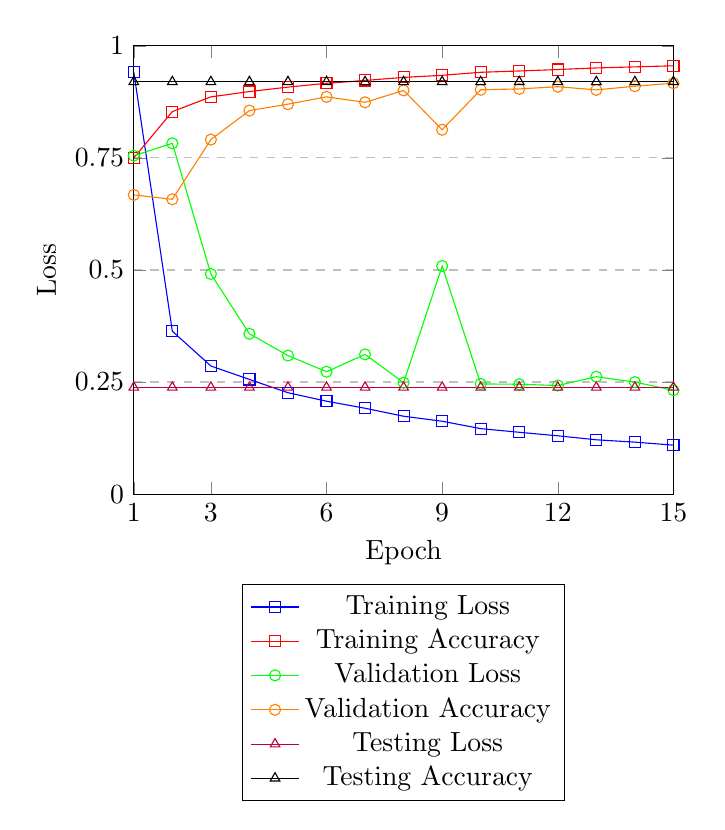
\begin{tikzpicture}
            \begin{axis}[
            xlabel={Epoch},
            ylabel={Loss},
            xmin=1, xmax=15,
            ymin=0, ymax=1,
            xtick={1, 3, 6, 9, 12, 15},
            ytick={0, .25, .50, .75, 1},
            legend style={at={(0.5,-0.2)},anchor=north},
            ymajorgrids=true,
            grid style=dashed,
            ]
                \addplot[
                color=blue,
                mark=square
                ]
                coordinates {
                (1, 0.9415369913395908)
                (2, 0.36347173816627926)
                (3, 0.2858551138391097)
                (4, 0.25580175934980315)
                (5, 0.22619957197457552)
                (6, 0.20731205224163002)
                (7, 0.19158202114825448)
                (8, 0.17376136417604154)
                (9, 0.1625804718480342)
                (10, 0.14612651362808216)
                (11, 0.1379509448694686)
                (12, 0.13010555795497364)
                (13, 0.12118976314862569)
                (14, 0.11594720014060537)
                (15, 0.10928217275068164)
                };
                \addplot[
                color=red,
                mark=square
                ]
                coordinates {
                (1, 0.7498944)
                (2, 0.8532715)
                (3, 0.8860656)
                (4, 0.8979578)
                (5, 0.90786415)
                (6, 0.9164315)
                (7, 0.9227066)
                (8, 0.9295607)
                (9, 0.9342024)
                (10, 0.94093925)
                (11, 0.94384027)
                (12, 0.9471116)
                (13, 0.9506346)
                (14, 0.9530575)
                (15, 0.9554094)
                };
                \addplot[
                color=green,
                mark=o
                ]
                coordinates {
                (1, 0.7549296505749226)
                (2, 0.7825332581996918)
                (3, 0.4910720940679312)
                (4, 0.357665928080678)
                (5, 0.3090804498642683)
                (6, 0.27299756929278374)
                (7, 0.31170774064958096)
                (8, 0.2485608123242855)
                (9, 0.508794916793704)
                (10, 0.24579987488687038)
                (11, 0.2450892459601164)
                (12, 0.24228437338024378)
                (13, 0.2619198402389884)
                (14, 0.24979994911700487)
                (15, 0.23182532005012035)
                };
                \addplot[
                color=orange,
                mark=o
                ]
                coordinates {
                (1, 0.66744876)
                (2, 0.6575944)
                (3, 0.79087156)
                (4, 0.8555428)
                (5, 0.86985517)
                (6, 0.88613117)
                (7, 0.8739339)
                (8, 0.9004858)
                (9, 0.81274575)
                (10, 0.901945)
                (11, 0.9038338)
                (12, 0.9087785)
                (13, 0.9017017)
                (14, 0.90983397)
                (15, 0.91657144)
                };
                \addplot[mark=triangle, color=purple]
                coordinates {
                (1, 0.23809038553127024)
                (2, 0.23809038553127024)
                (3, 0.23809038553127024)
                (4, 0.23809038553127024)
                (5, 0.23809038553127024)
                (6, 0.23809038553127024)
                (7, 0.23809038553127024)
                (8, 0.23809038553127024)
                (9, 0.23809038553127024)
                (10, 0.23809038553127024)
                (11, 0.23809038553127024)
                (12, 0.23809038553127024)
                (13, 0.23809038553127024)
                (14, 0.23809038553127024)
                (15, 0.23809038553127024)
                };
                \addplot[mark=triangle, color=black]
                coordinates {
                (1, 0.9196472)
                (2, 0.9196472)
                (3, 0.9196472)
                (4, 0.9196472)
                (5, 0.9196472)
                (6, 0.9196472)
                (7, 0.9196472)
                (8, 0.9196472)
                (9, 0.9196472)
                (10, 0.9196472)
                (11, 0.9196472)
                (12, 0.9196472)
                (13, 0.9196472)
                (14, 0.9196472)
                (15, 0.9196472)
                };
                \legend{Training Loss, Training Accuracy, Validation Loss, Validation Accuracy, Testing Loss, Testing Accuracy}
            \end{axis}
        \end{tikzpicture}
    \end{figure}

    \subsection{Testing}\label{subsec:testing}

    The trained model was evaluated over all 128 testing images plus one extra that I will explain in the conclusion section.\ The testing loss and accuracy are reported in~\autoref{fig:loss-and-accuracy}.

    \subsection{Post-processing}\label{subsec:post-processing}

    Once the model was trained and evaluated against the testing data, it was used to predict segmentation trimaps for each of the testing images.\ Of course, the predicted trimaps were normalized to the network's output size of 150x150 pixels.\ These square outputs look distorted when compared to the original X-rays, so each was resized to the original dimensions of its respective testing image.

    While input X-rays could now be compared with their predicted trimaps, it became obvious that interlacing the two would yield a superior visualization.\ By leveraging ImageMagick techniques as demonstrated in this discussion~\cite{image-magick}, each of the testing image trimaps was interlaced with its input image.\ In between, each trimap had to be converted from the predicted representation using three distinguishable colors (black, gray, and white) to an intermediate trimap representation using the three darkest shades of black (1, 2, and 3 in rgb coordinates).\ This conversion produces a trimap that is compatible with ImageMagick, though it is impossible to distinguish between the shades of black visually.\ Each of the final interlaced images was saved to disk.

    \section{Results}\label{sec:results}

    The two metrics used to evaluate the model's ability to learn are loss and accuracy.\ The predictions it made yielded a loss rate of 24\% and an accuracy of 92\% when compared against the hand-drawn trimaps.\ These metrics are likely insufficient for real-world application when compared against human performance.\ While a metric tracking human performance at spine segmentation could not be identified, I expect it to be higher than the model's performance.\ Keep in mind, the ultimate goal of doing Cobb angle prediction has the potential for more competition as inter- and intra-person performance varies between 3--10\%\cite{doi:10.14245/ns.1938426.213} due to factors including image quality, professional experience, and time pressure.\ That problem retains promise for further research.

    The following figures visualize some unique challenges the model faced during training.\ As you can see in \autoref{fig:results4}, it successfully segments the spine through its extreme curvature, even surviving its encounter with the edge. \autoref{fig:results3} shows how it learns to segment the spine despite the presence of what appear to be Harrington rods surgically implanted to stabilize the spine;\ though, the predicted mask does appear to have included the upper screws of that mechanism. \autoref{fig:results} and \autoref{fig:results2} both demonstrate failure cases which would prevent Cobb angle prediction.\ In \autoref{fig:results}, it seems the obscuring organ results in a gap in the mask.\ To human eyes, the organ increases contrast, thus actually making it easier to identify the edges of the spine, but it seems the model cannot make that same conclusion.\ The gap in the predicted mask for \autoref{fig:results2} may also have been affected by an organ, though the necklace may have had a hand to play in the inaccuracy as well.

    Finally, I would like to draw special attention to the predicted mask shown in \autoref{fig:results5}.\ The model has segmented the spine quite well in this case.\ It is especially meaningful to me to see this result as it is, in fact, my own.
    
    \begin{figure}
        \caption{A test image and its masks}
        \label{fig:results}
        \centering
        \subfloat[\centering Input]{{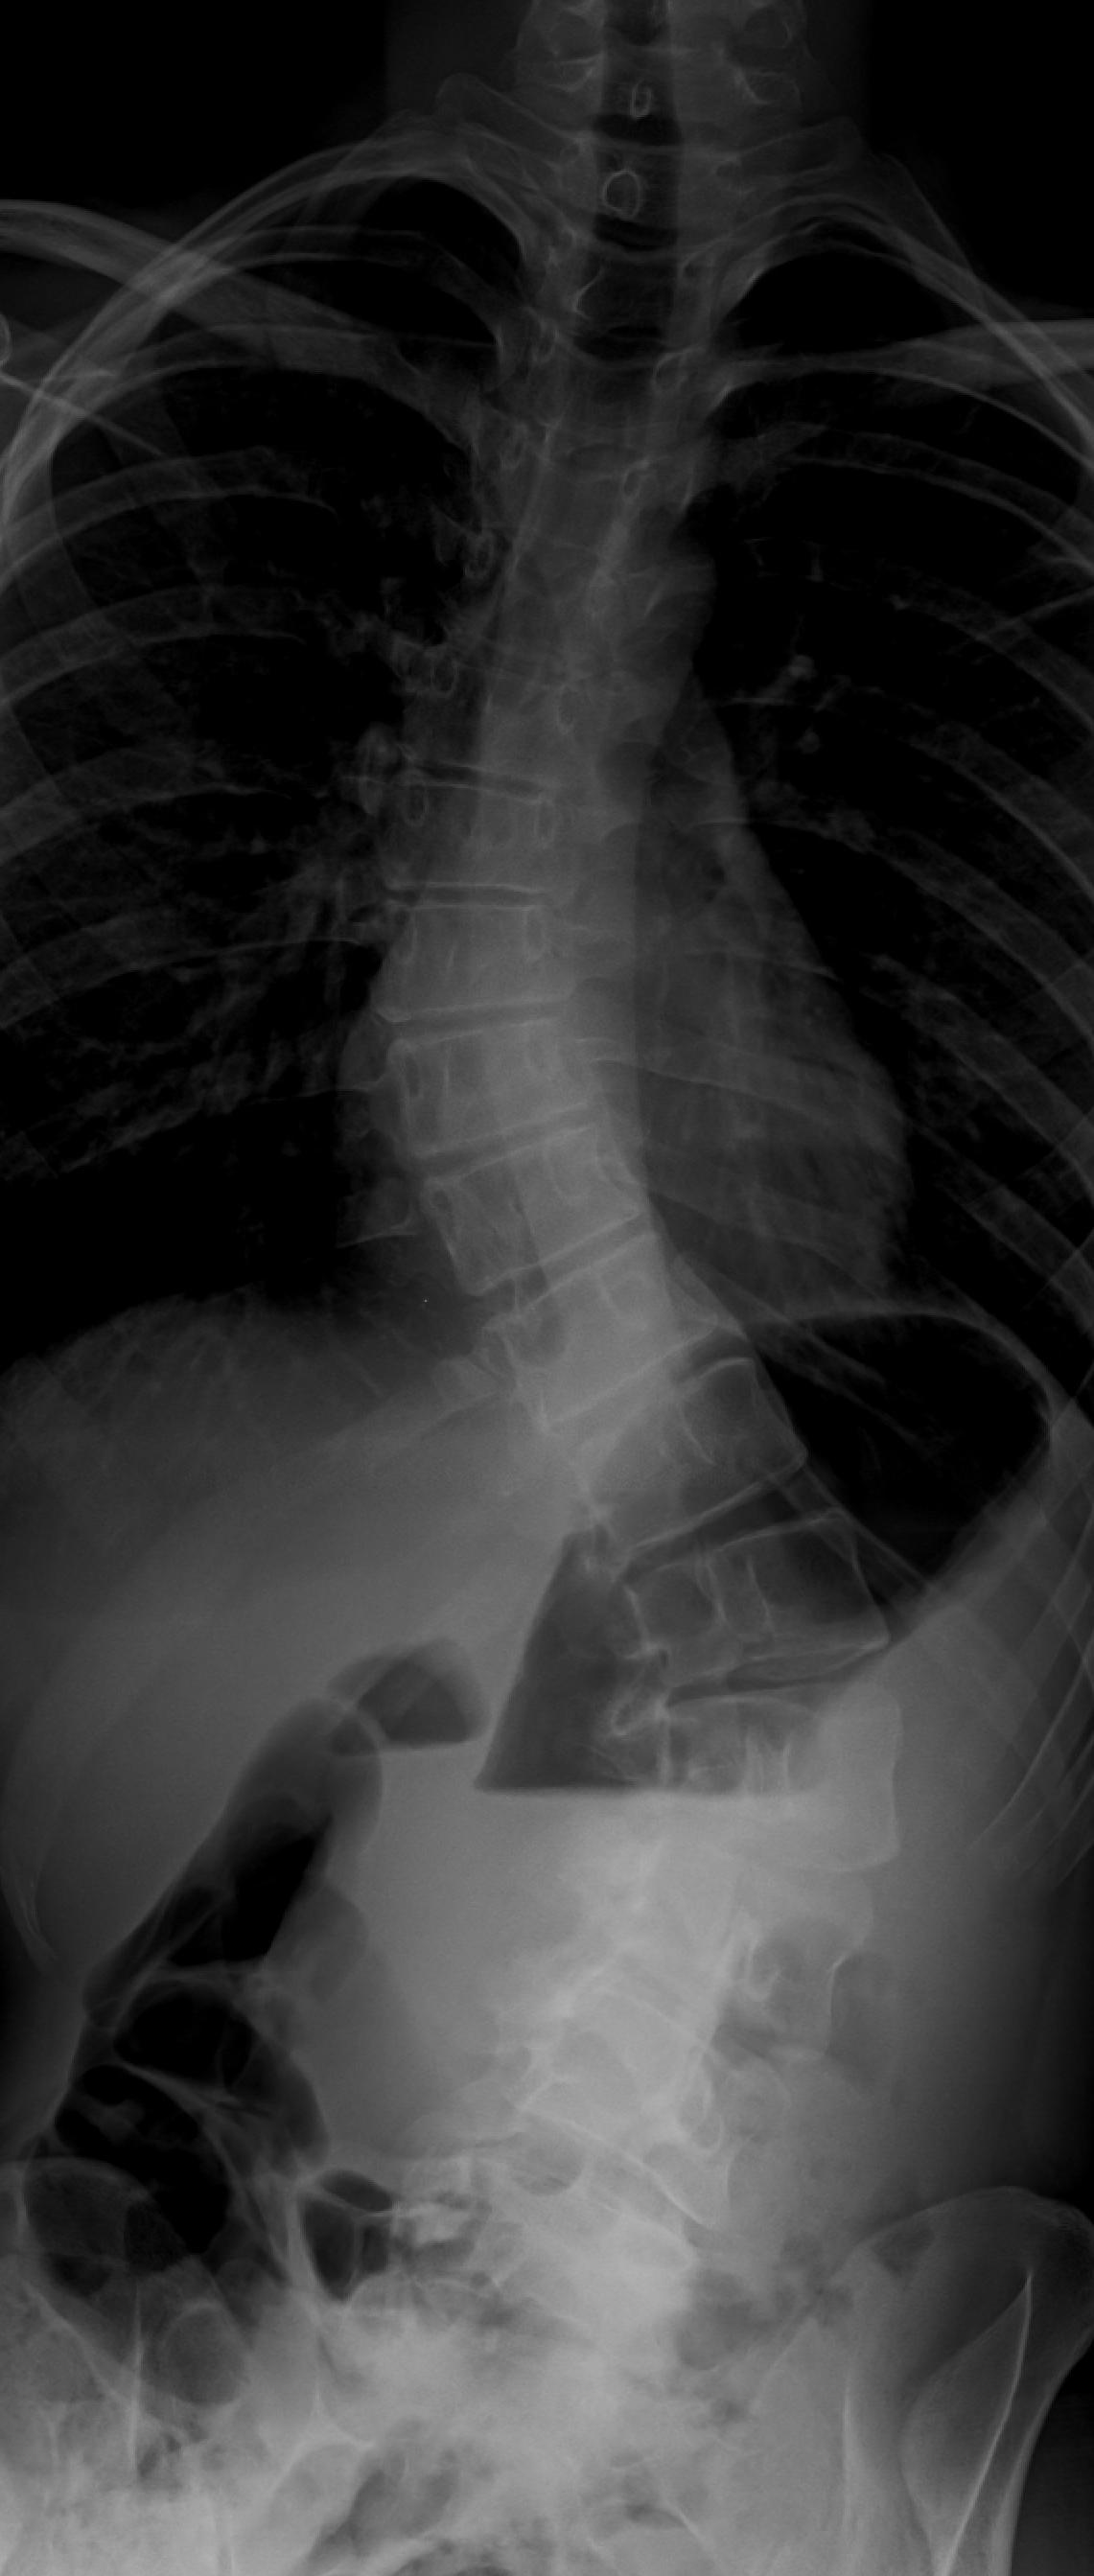
\includegraphics[width=2.75cm]{image32-input.jpg} }}
        \subfloat[\centering Mask]{{\includegraphics[width=2.75cm]{image32-mask.png} }}
        \subfloat[\centering Output]{{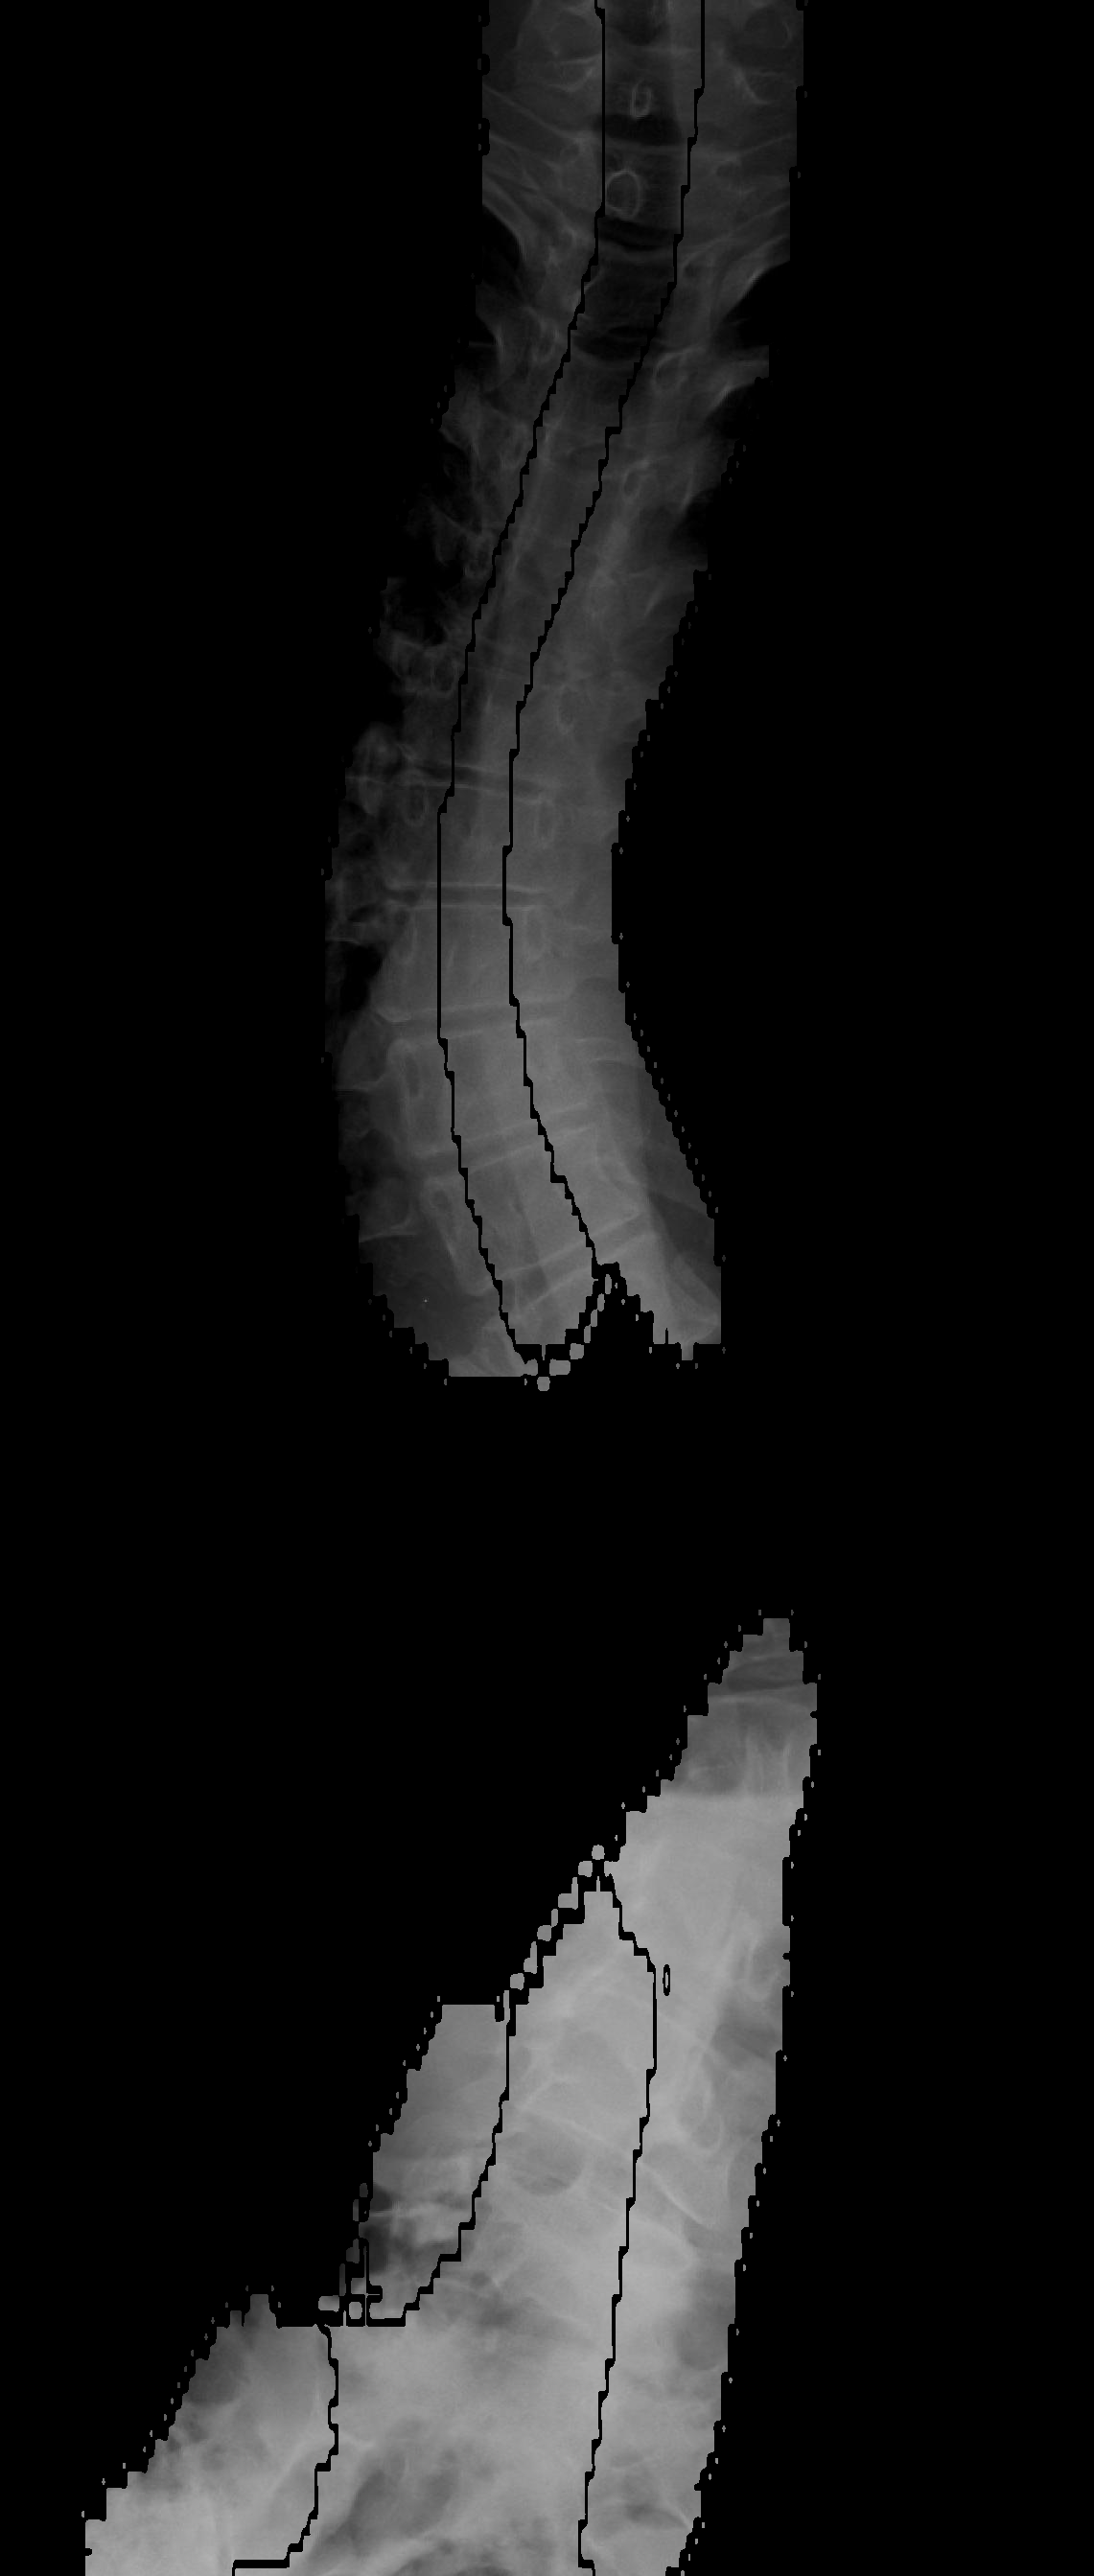
\includegraphics[width=2.75cm]{image32-output.png} }}
    \end{figure}

    \begin{figure}
        \caption{A test image and its masks}
        \label{fig:results2}
        \centering
        \subfloat[\centering Input]{{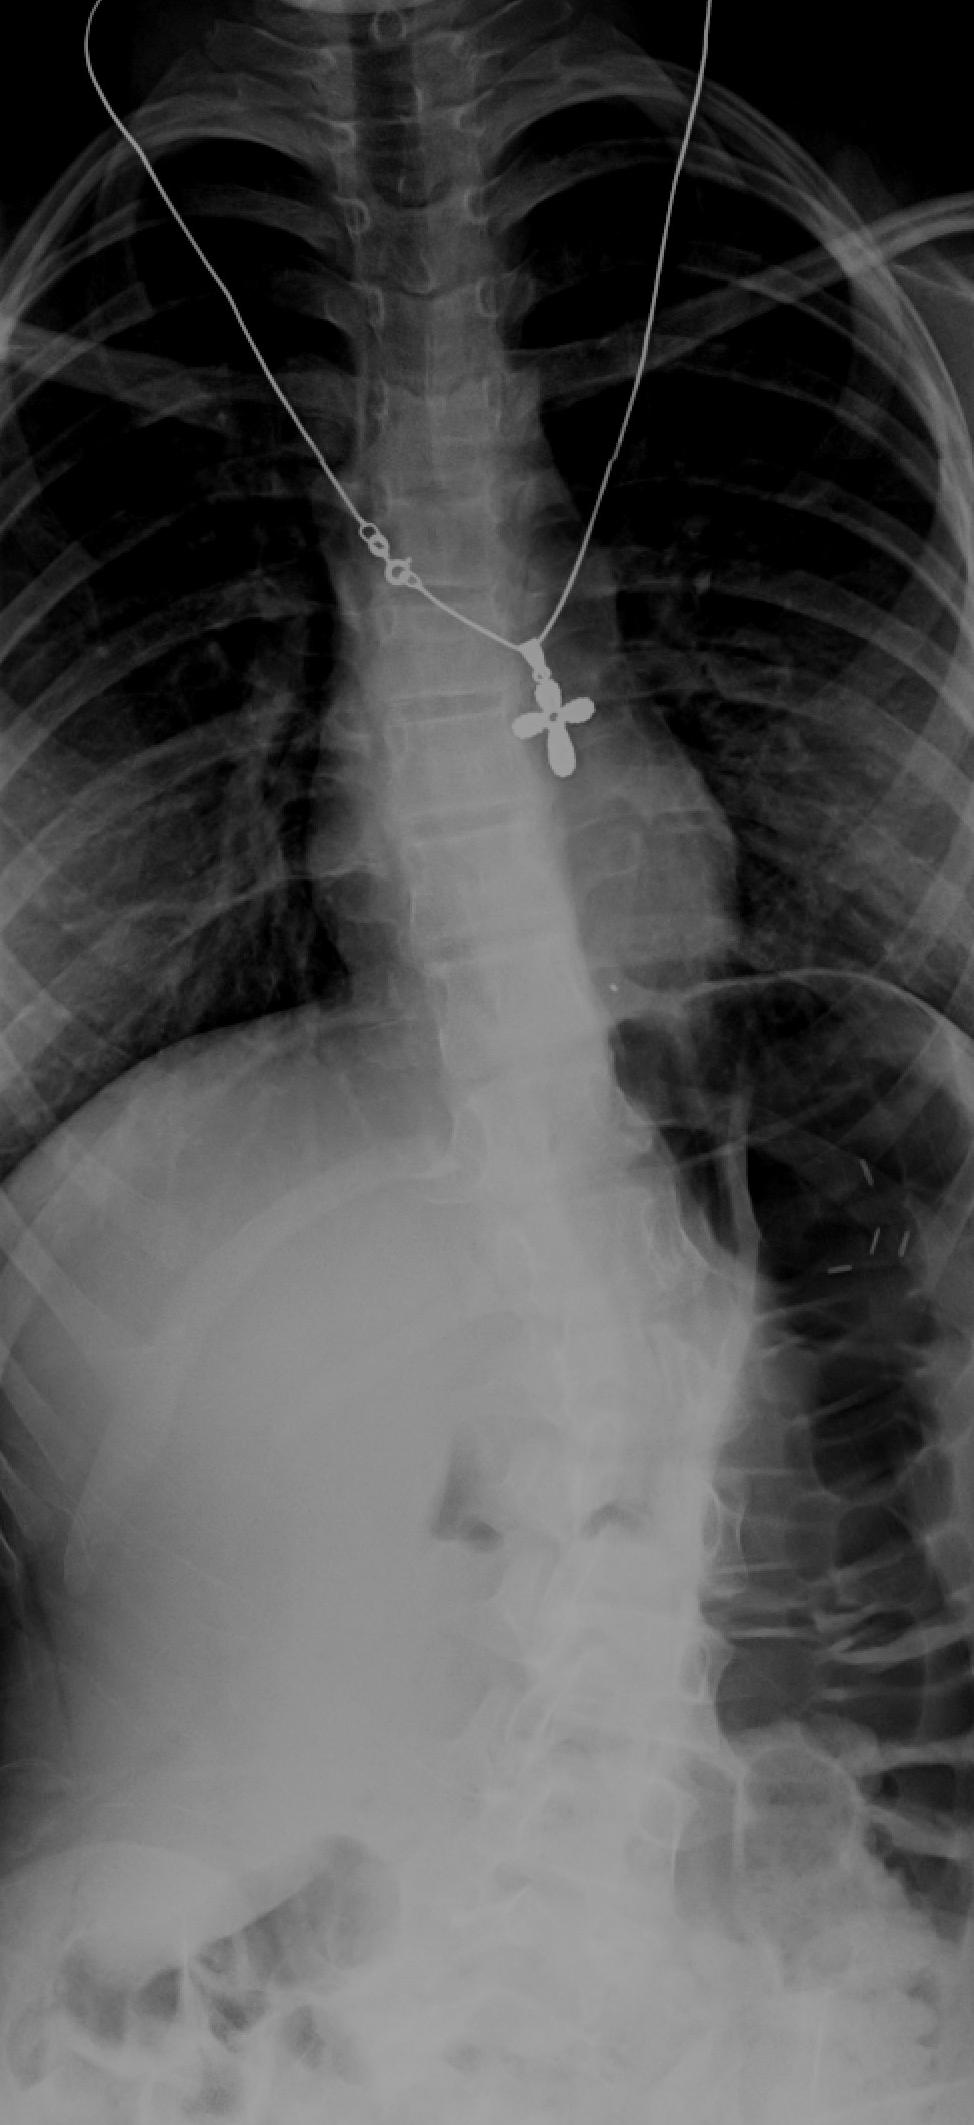
\includegraphics[width=2.75cm]{image61-input.jpg} }}
        \subfloat[\centering Mask]{{\includegraphics[width=2.75cm]{image61-mask.png} }}
        \subfloat[\centering Output]{{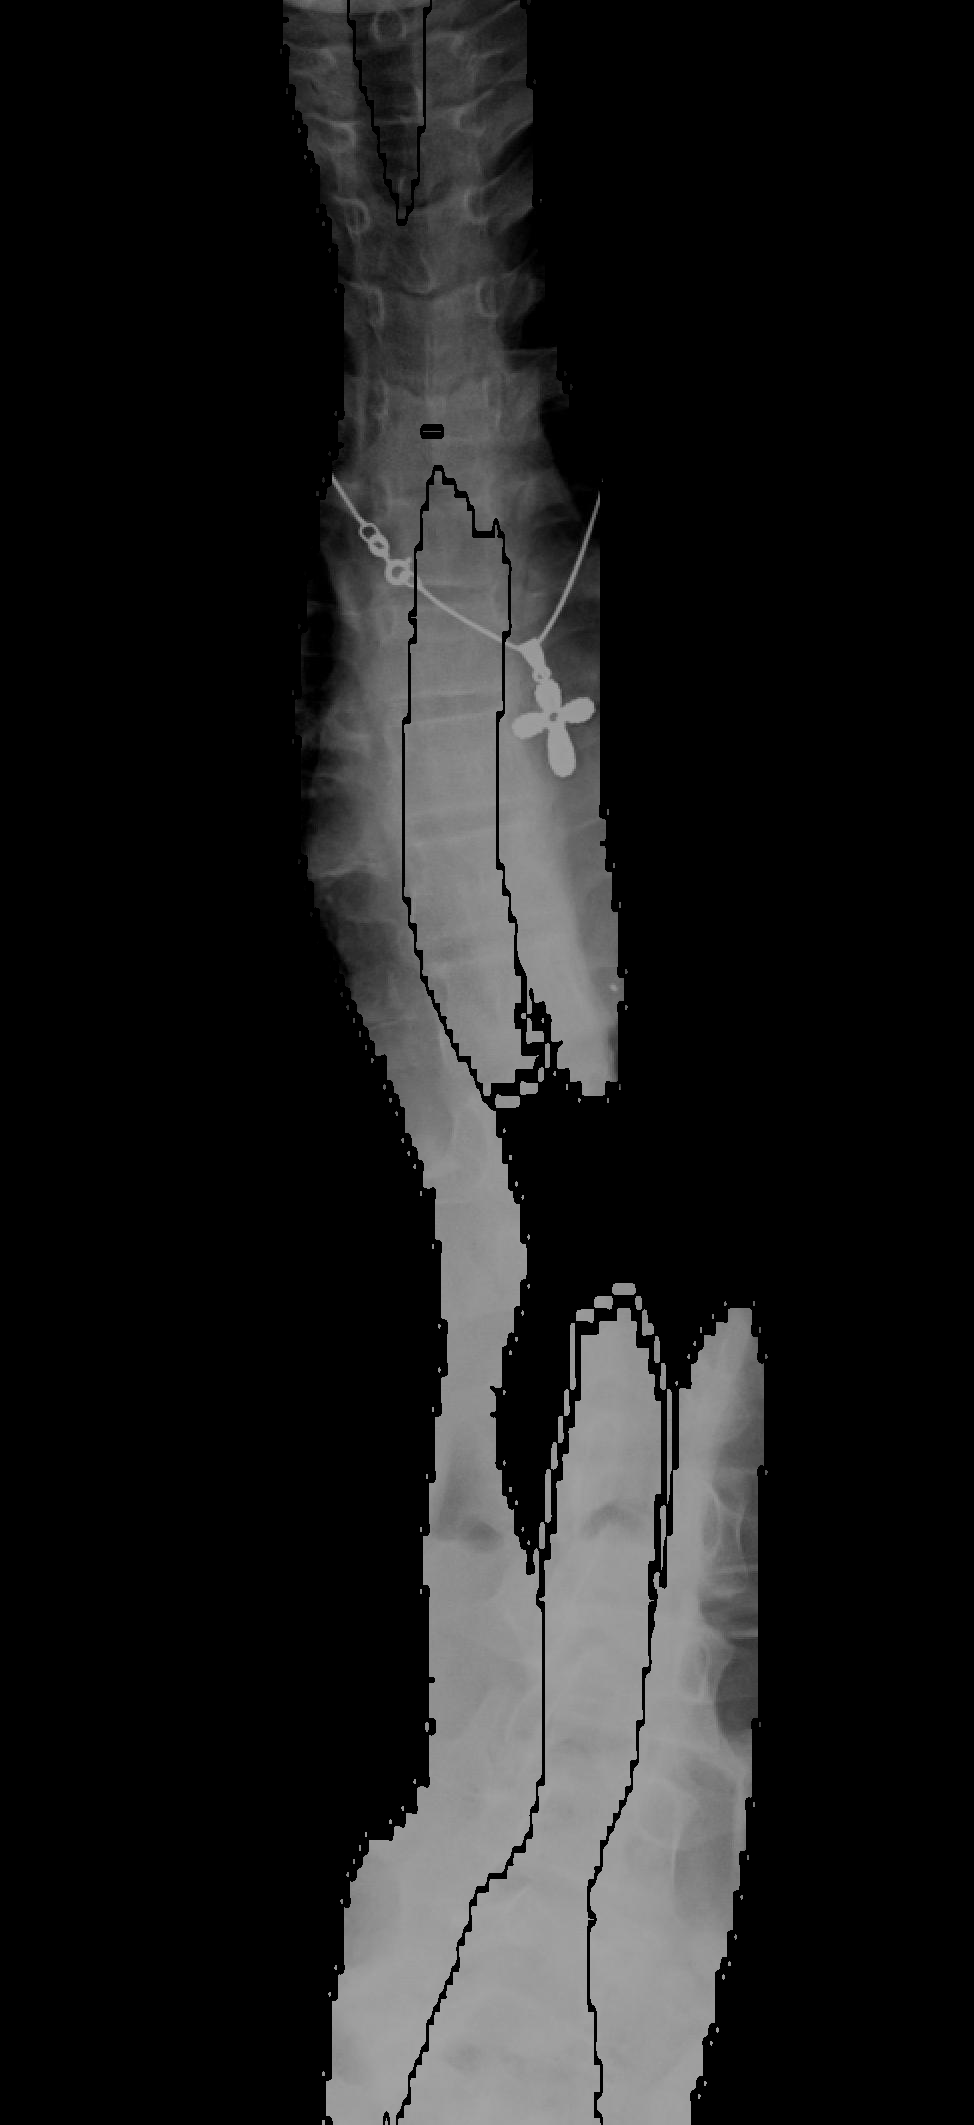
\includegraphics[width=2.75cm]{image61-output.png} }}
    \end{figure}

    \begin{figure}
        \caption{A test image and its masks}
        \label{fig:results3}
        \centering
        \subfloat[\centering Input]{{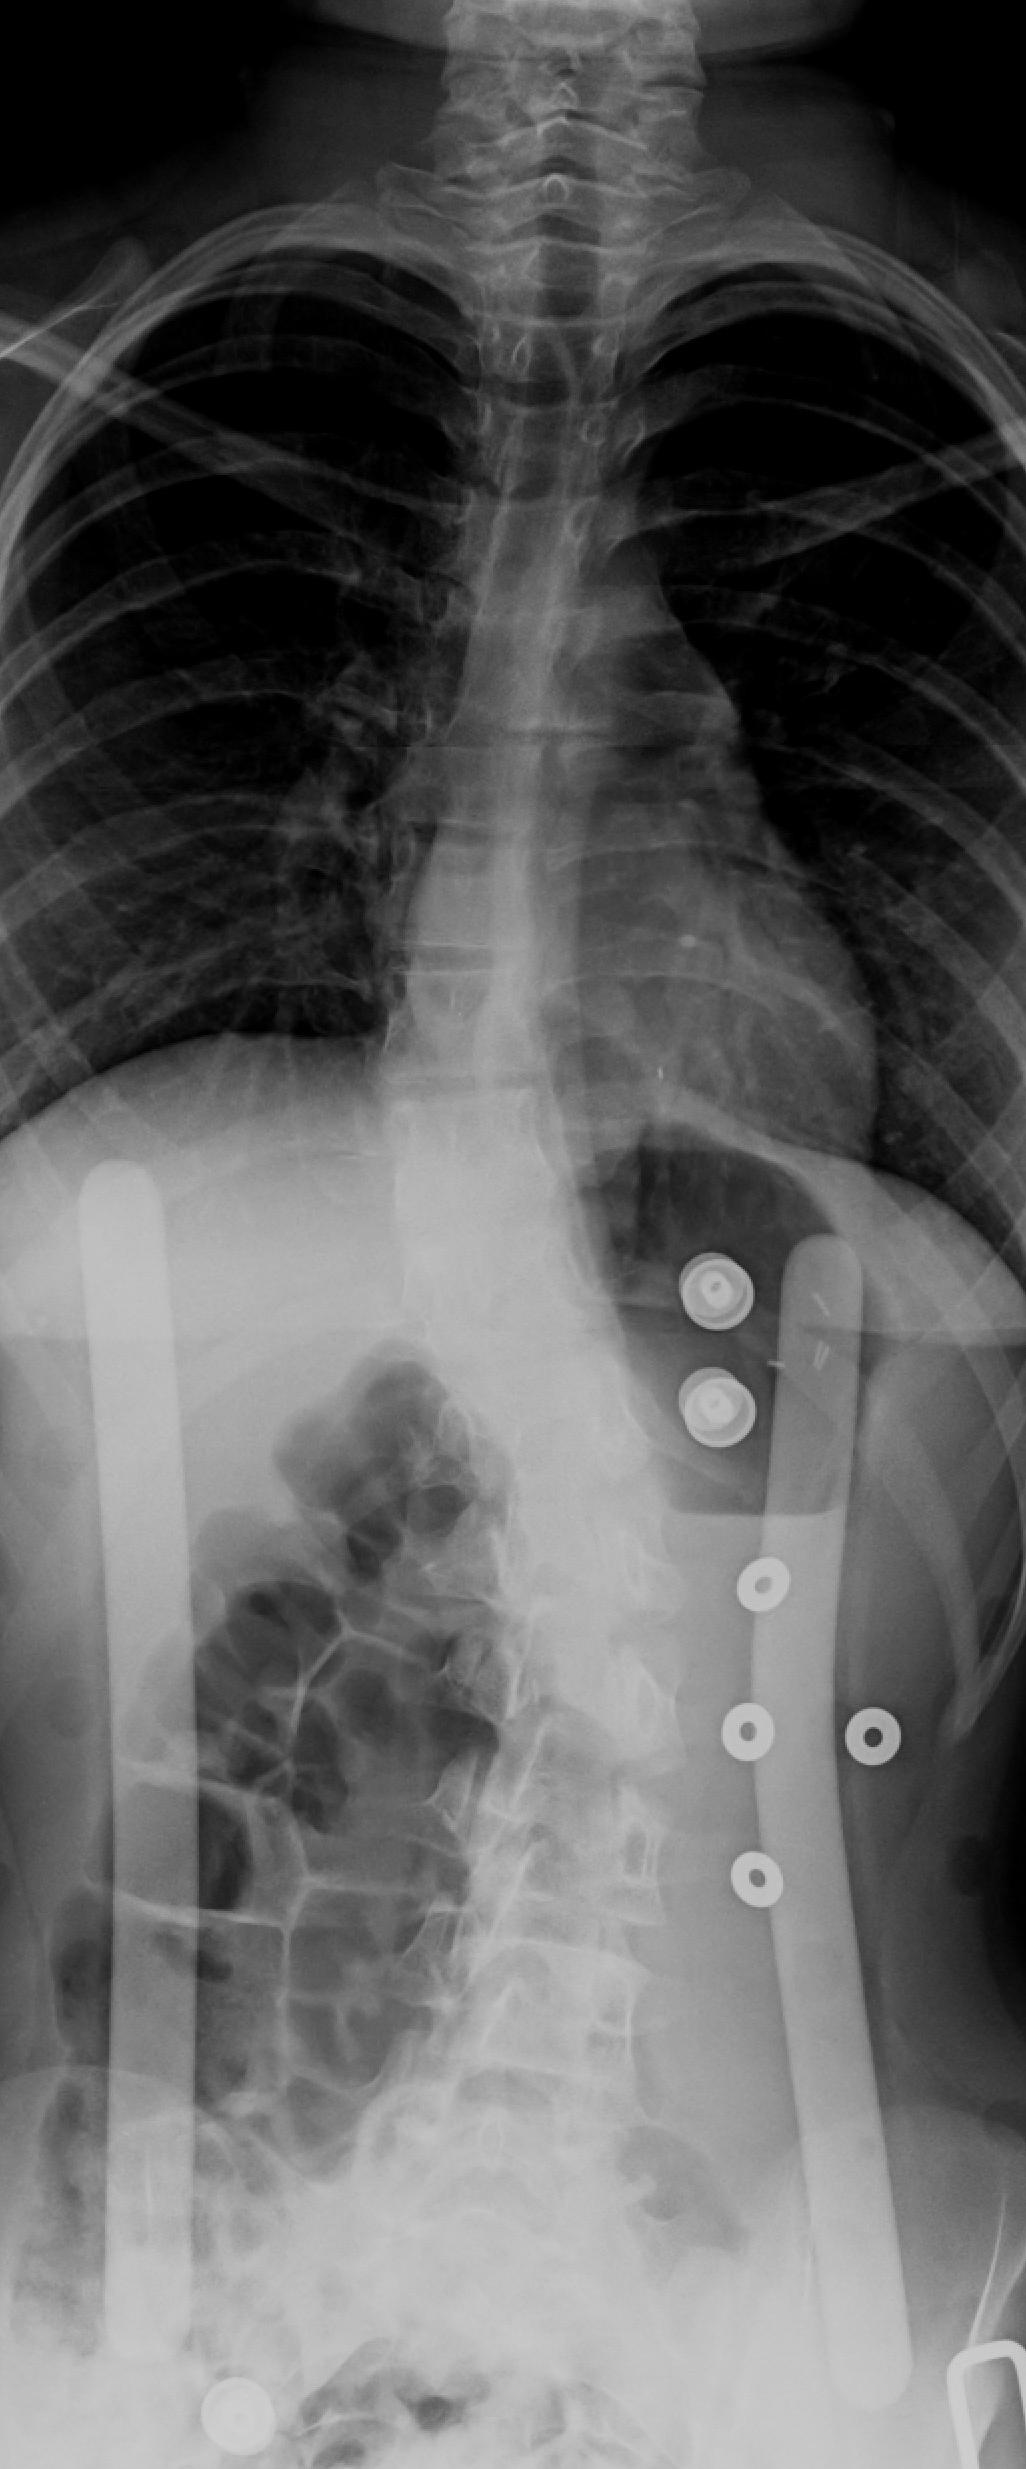
\includegraphics[width=2.75cm]{image63-input.jpg} }}
        \subfloat[\centering Mask]{{\includegraphics[width=2.75cm]{image63-mask.png} }}
        \subfloat[\centering Output]{{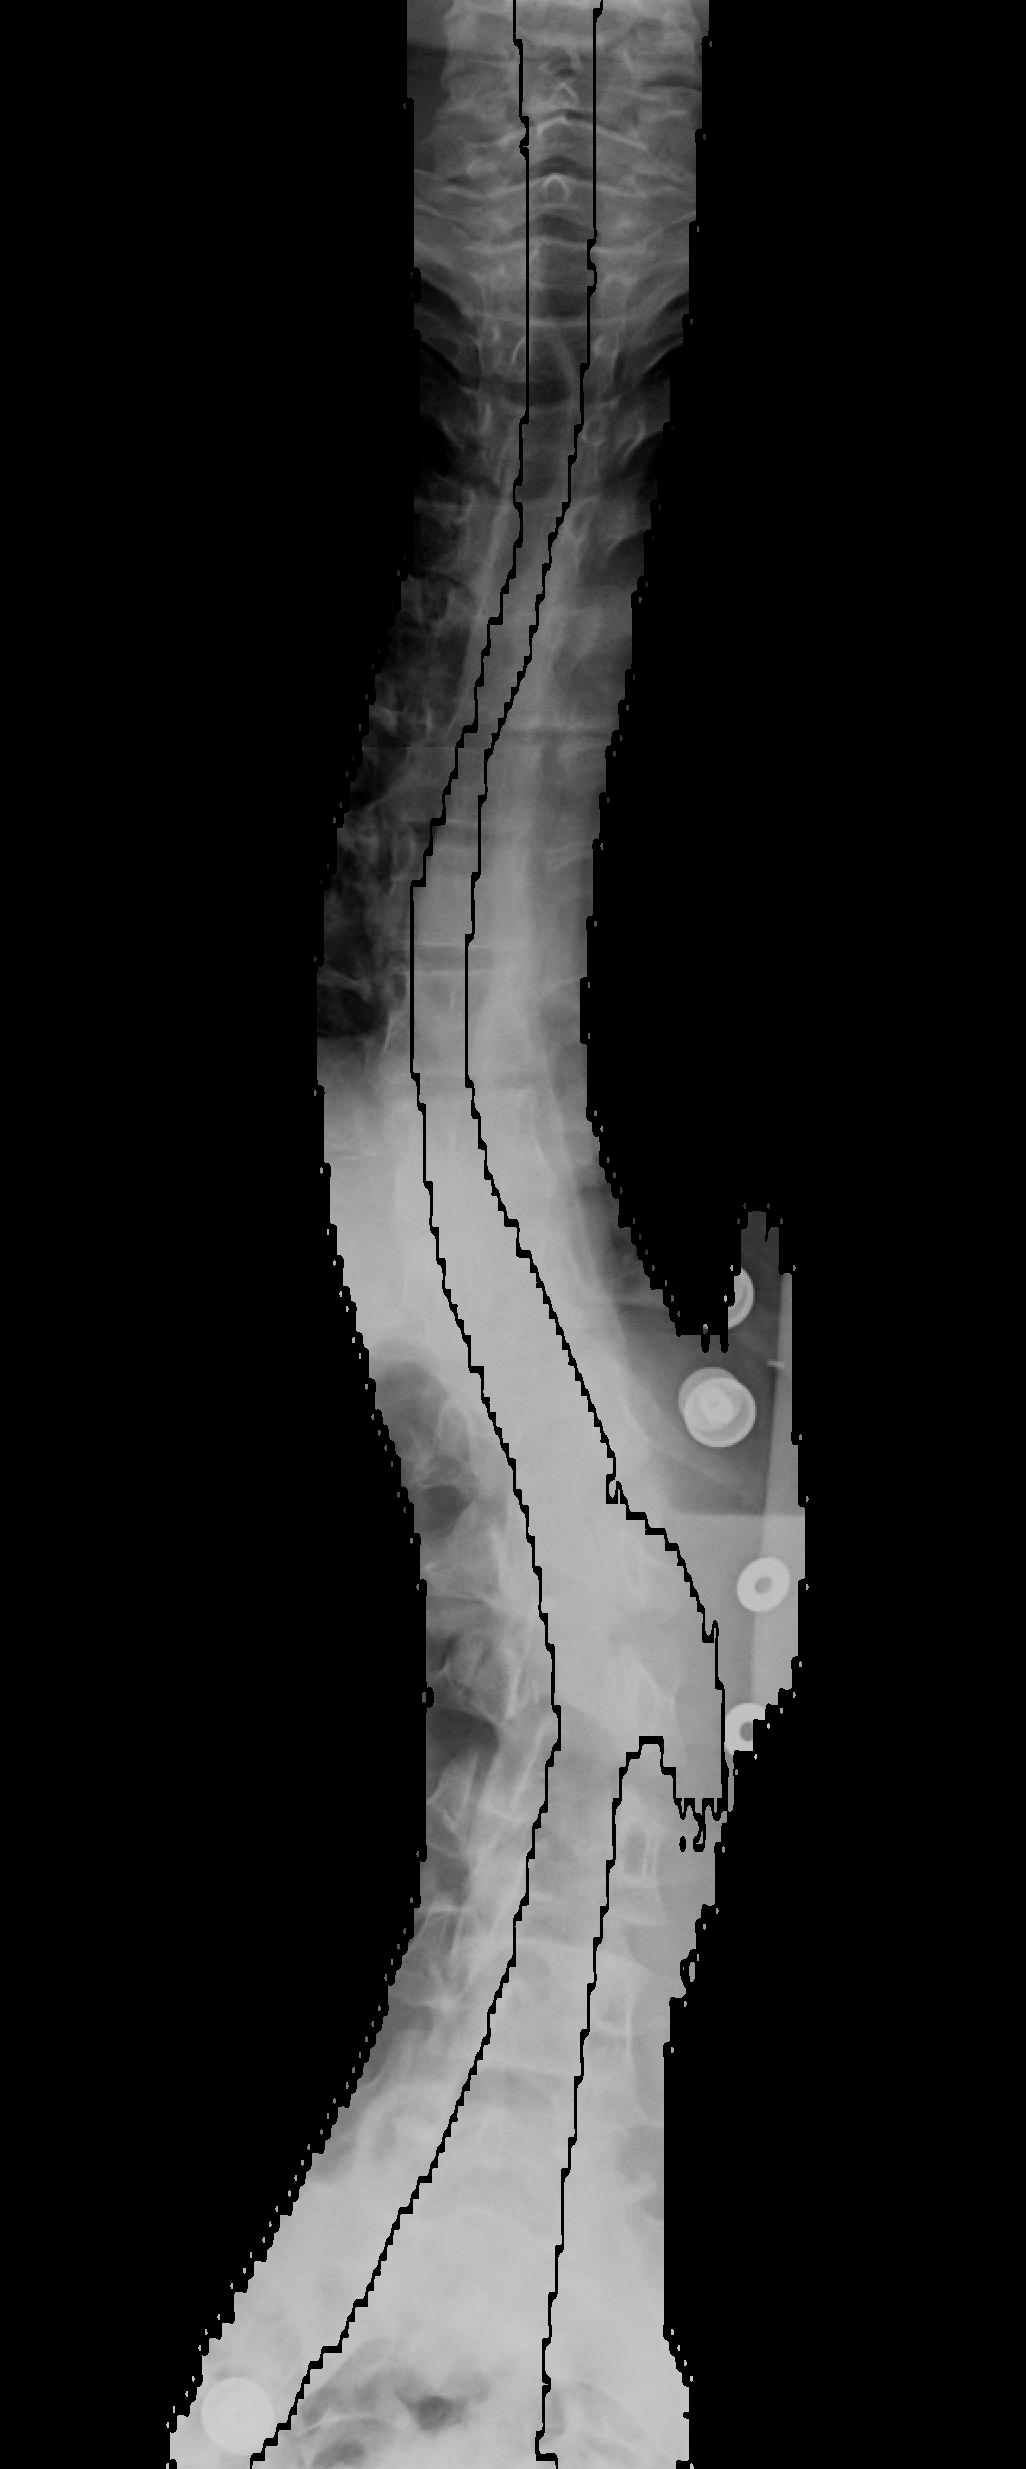
\includegraphics[width=2.75cm]{image63-output.png} }}
    \end{figure}

    \begin{figure}
        \caption{A test image and its masks}
        \label{fig:results4}
        \centering
        \subfloat[\centering Input]{{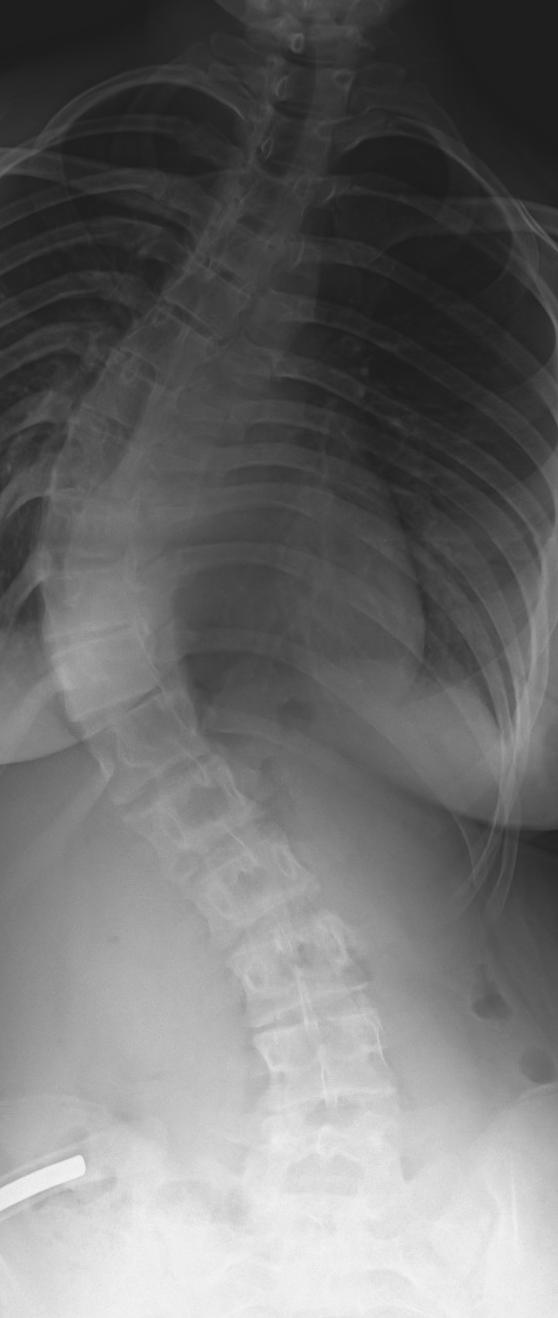
\includegraphics[width=2.75cm]{image70-input.jpg} }}
        \subfloat[\centering Mask]{{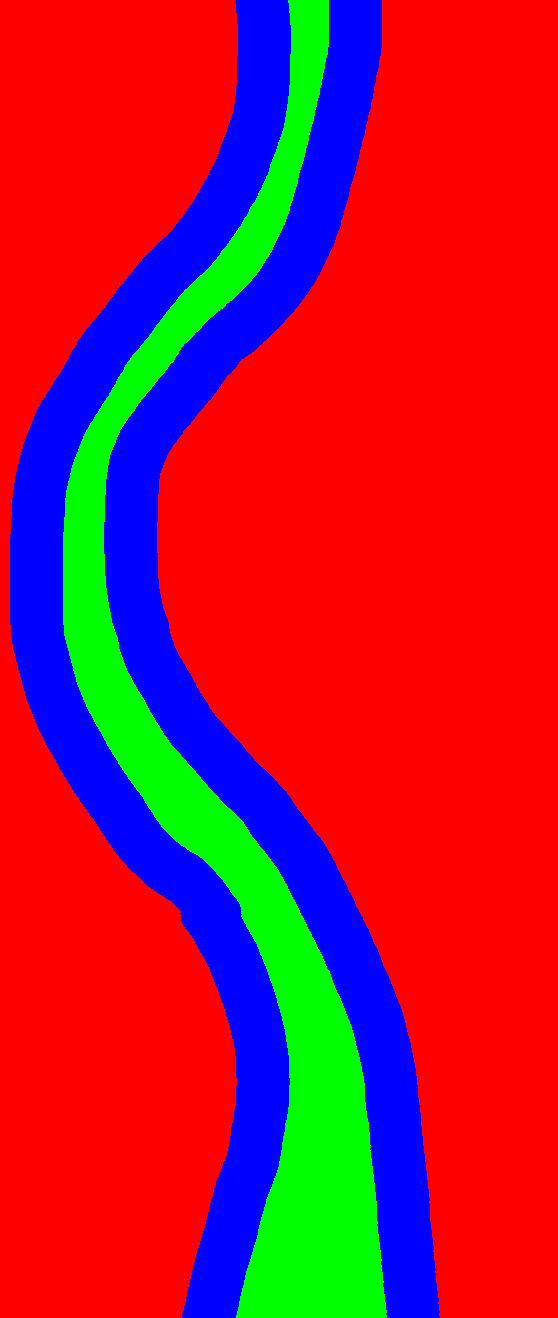
\includegraphics[width=2.75cm]{image70-mask.png} }}
        \subfloat[\centering Output]{{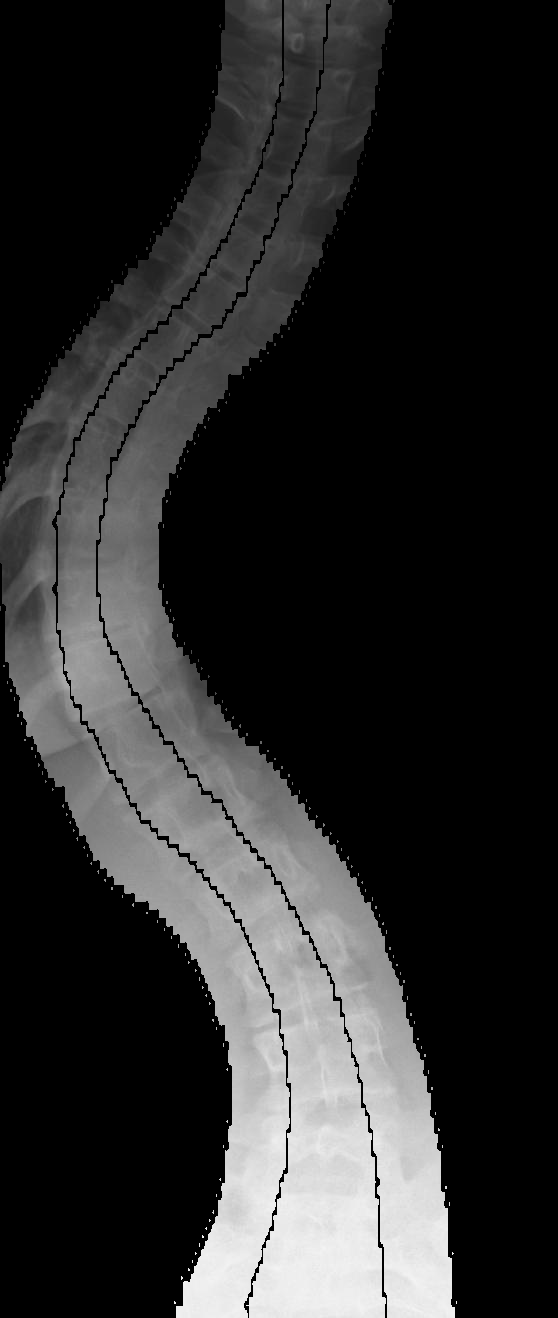
\includegraphics[width=2.75cm]{image70-output.png} }}
    \end{figure}

    \begin{figure}
        \caption{A test image and its masks}
        \label{fig:results5}
        \centering
        \subfloat[\centering Input]{{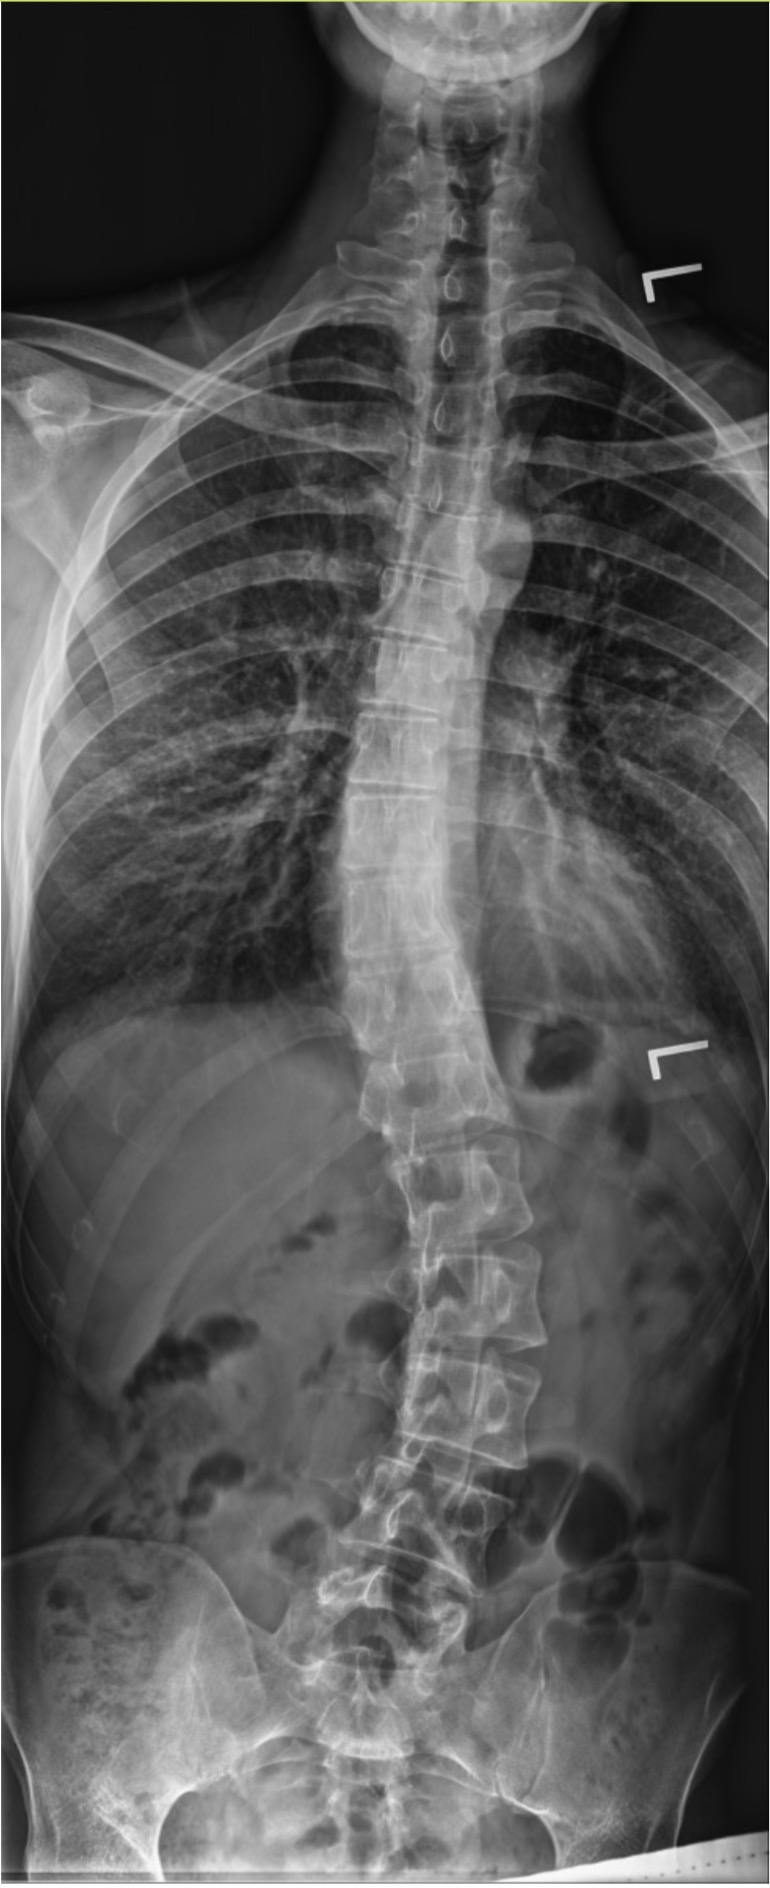
\includegraphics[width=2.75cm]{image128-input.jpg} }}
        \subfloat[\centering Mask]{{\includegraphics[width=2.75cm]{image128-mask.png} }}
        \subfloat[\centering Output]{{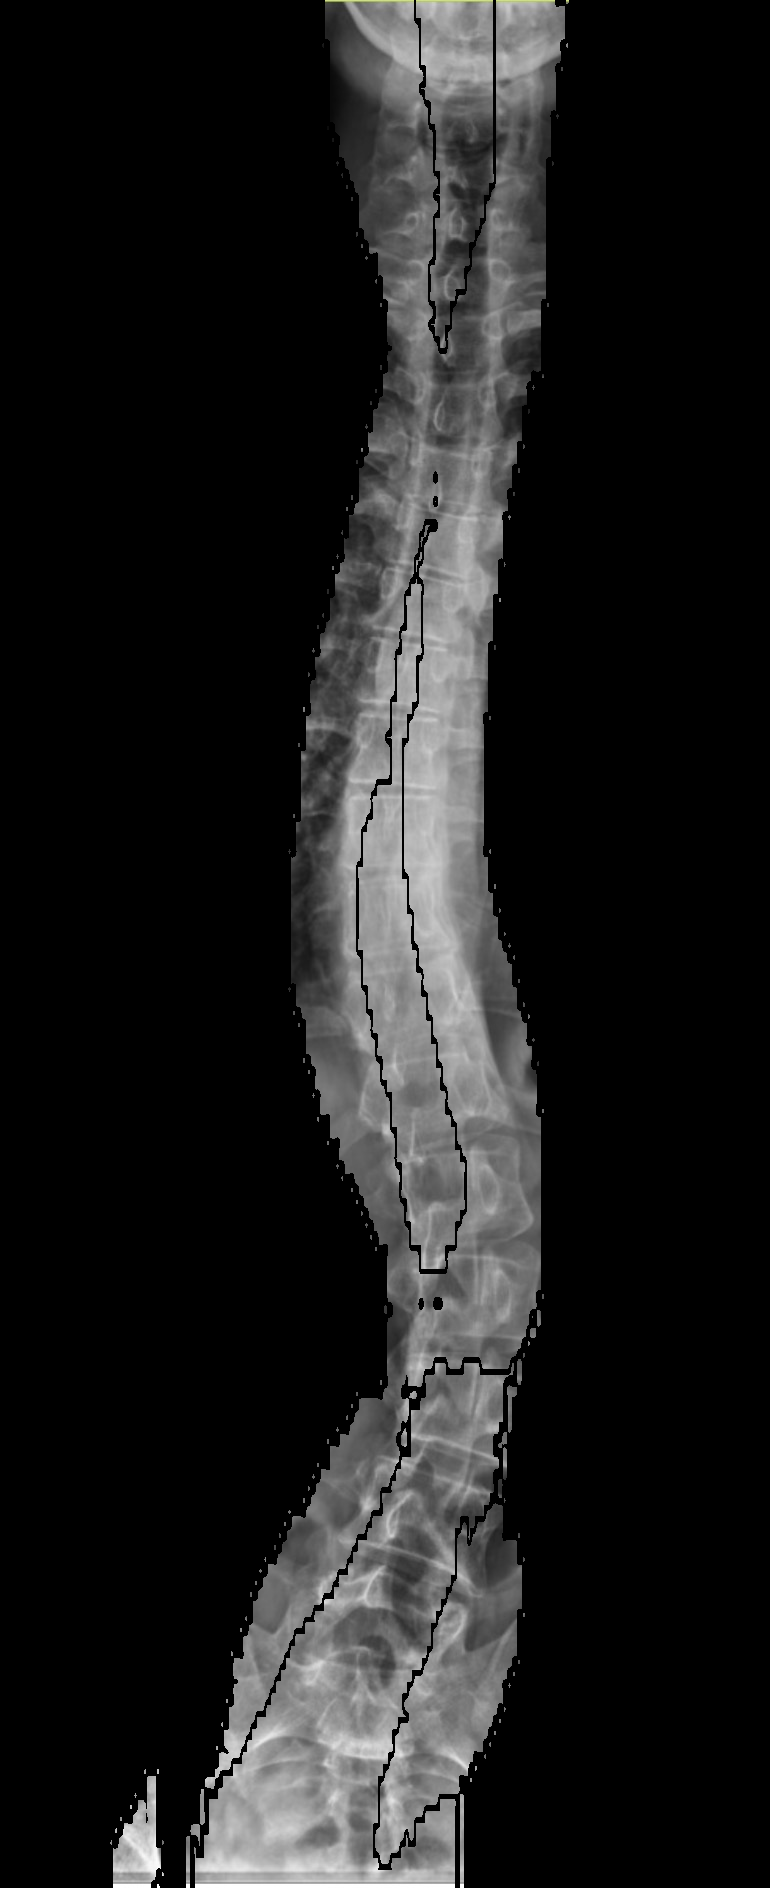
\includegraphics[width=2.75cm]{image128-output.png} }}
    \end{figure}

    \section{Conclusion}\label{sec:conclusion}

    The ability to segment the spine from a posteroanterior X-ray with 92\% accuracy is an encouraging first step toward the ultimate goal of Cobb angle prediction.\ Next semester, I intend to build upon this work in the Deep Learning course by training a model to detect the individual vertebrae in segmented spine images.\ For now, I conclude with gratitude to Dr. Mahima Agumbe Suresh for educating me in the fundamentals of machine learning.

    \bibliographystyle{ieeetr}
    \bibliography{report}
\end{document}